\chapter{Generative Adversarial Networks - Améliorations}


\section{Apprentissage par Mini-Batch}
\subsection{Principe}
L'apprentissage par Batch consiste à apprendre sur l'ensemble du batch d'apprentissage avant de mettre à jour chaque réseau, et de réitérer l'apprentissage à chaque itération sur l'ensemble du batch d'apprentissage. Il s'oppose à l'apprentissage habituel, dit \textit{stochastique} (mais qui n'a rien de particulièrement stochastique), qui consiste à rétropropager l'erreur et mettre à jour les poids image par image.

On calcule successivement la rétropropagation pour chaque image, on somme l'erreur sur l'ensemble des images et on applique la mise à jour du réseau avec la somme des erreurs. On obtient donc une moyenne des directions de propagation afin d'effectuer la mise à jour, afin de converger de manière plus précise.

Certaines bases d'apprentissage étant très grandes - soixante mille avec MNIST par exemple -, on va préférer à l'apprentissage par batch, l'apprentissage par minibatch. 
On sélectionne aléatoirement parmi la base d'apprentissage et de tests un nombre plus petit d'éléments. Les valeurs sont habituellement de l'ordre de la dizaine d'éléments.
\subsection{Implémentation}
\paragraph{Mise à jour des poids}
Afin de pouvoir effectuer la rétro-propagation uniquement à la fin de l'itération du minibatch, nous avons simplement 

\paragraph{Sets d'apprentissage et de tests. plus petits}
Dans le cas de MNIST, les chiffres du début de la base d'apprentissage étant plus simple, nous avons, afin d'obtenir de meilleurs résultats, parfois effectué une sélection aléatoire sur uniquement une première partie des 60000 images d'apprentissage (cf argument \textit{labelTrainSize} du fichier de configuration \cite{barrios_gan_2018}) et des 10000 images de tests (cf argument \textit{labelTestSize}.

\subsection{Résultats}
Notre équipe a obtenu des résultats corrects mais peu intéressant, et très différents des résultats relativement exotiques du groupe Salamandre \cite{bouvier_dyvoire_dessine-moi_2018}.
Globalement, l'apprentissage s'effectue légèrement plus rapidement pour un même nombre d'itérations, au prix d'une augmentation du temps de calcul par itération (proportionnel selon la taille des batch). Le temps de calcul était donc quasiment multiplié par la taille du batch pour un résultat équivalent en stochastique (voire pire dans le cas du minibatch 1, l'apprentissage stochastique ayant par ailleurs été optimisé, comme on peut le remarquer sur la figure ci-dessous en comparant la courbe orange de la jaune).

La technique de minibatch, bien qu'intéressante dans des cas précis, tel que l'apprentissage simultané de plusieurs chiffres au même temps, a donc été par la suite abandonnée.

\begin{figure}[h]
\begin{center}
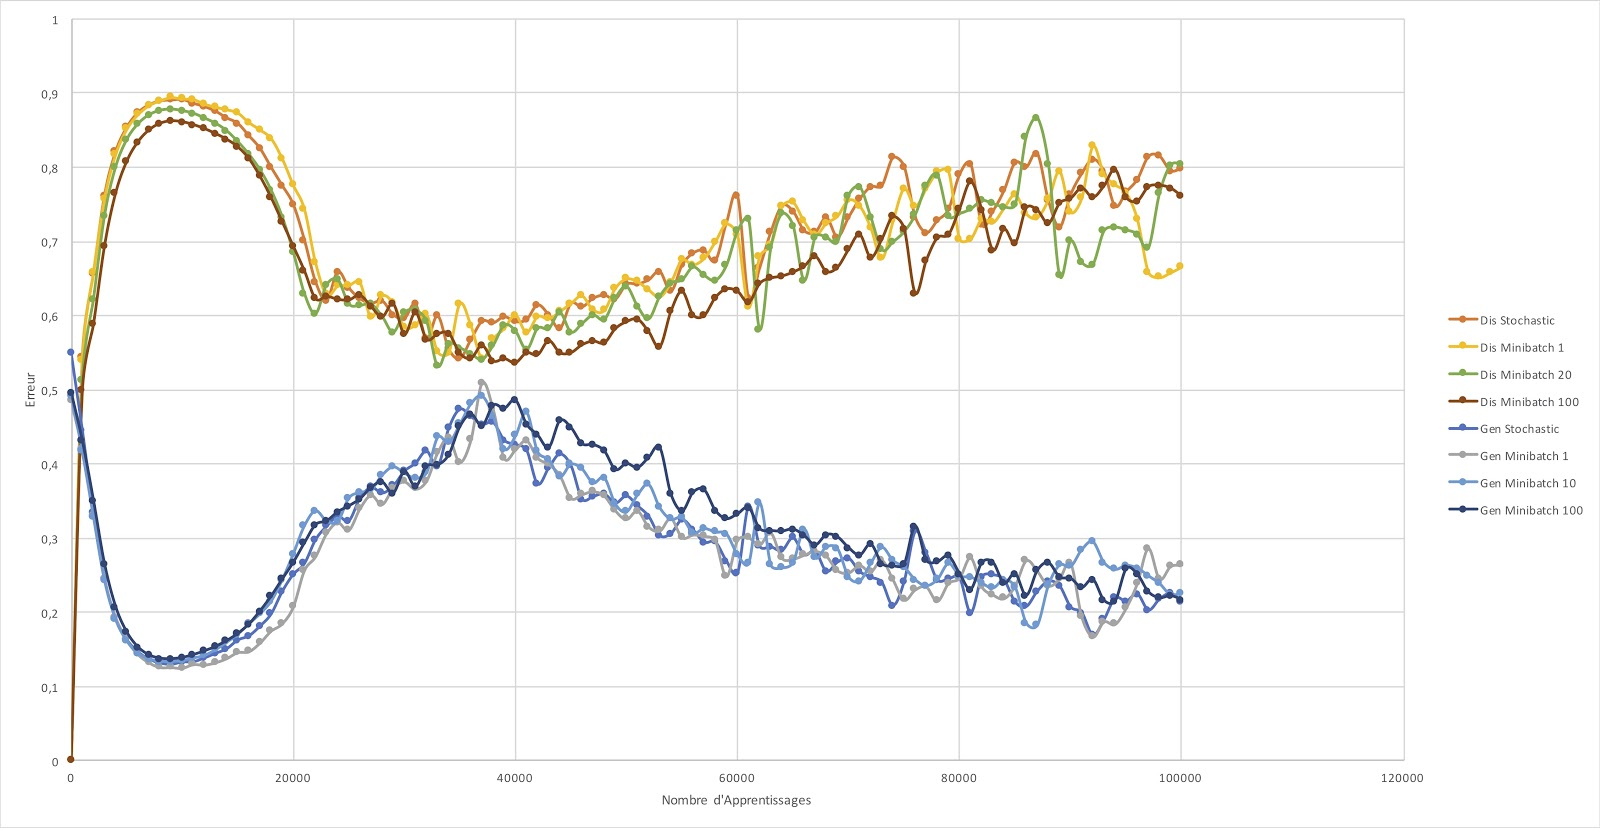
\includegraphics[width=1\textwidth]{images/08-gan_ameliorations_resultats_1.jpg}\caption{Apprentissage par minibatch 100 (marron et gris) et minibatch 10 (vert et cyan) d'un GAN sur MNIST comparé à un apprentissage stochastique (orange et bleu clair)}
\end{center}
\end{figure} 



\section{Algorithmes de pas d'apprentissage adaptatif}
\subsection{Principe}
L'objectif de ces algorithmes est de paramétrer au mieux la convergence de la distribution représentée par notre réseau vers la distribution $p_data$. Le pas adaptatif n'est alors plus constant; il varie en fonction du gradient des étapes d'apprentissage précédentes, de manière plus ou moins évoluée selon les algorithmes.

L'objectif est ainsi de faire évoluer le pas en fonction des erreurs, selon diverses formules. Deux méthodes de pas adaptatifs ont été utilisées : RMSprop et Adam. Nous en présentons ici d'autres.

\subsection{Adagrad}

Cette première méthode de descente adaptative suit les équations suivantes :

\begin{equation}
\begin{aligned}
g_{t+1} = g_t + (\frac{\partial J}{\partial W})^2 \\
W_{t+1} = W_t - \dfrac{\eta}{\sqrt{g_{t+1}} + \epsilon}\frac{\partial J}{\partial W}
\end{aligned}
\end{equation} 

Adagrad n'a pas été implémenté en raison des piètres performances annoncées \cite{ruder_overview_2016}. En effet, g est strictement croissante, étant incrémenté à chaque itération de $(\frac{\partial J}{\partial W})^2$ . Les réseaux apprenant sur un grand nombre d'itération, le coefficient $g_{t}$ devient rapidement très important, et le pas en $\dfrac{1}{\sqrt{g_{t+1}}}$ devient rapidement négligeable. Les performances de cet algorithme sont donc assez faibles.

\subsection{RMSprop}

La RMSProp permet de résoudre ce problème. En effet, on a un décroissance exponentielle de l'influence de l'erreur dans le temps grâce au coefficient $\gamma$ correspondant au moment d'ordre 2. Ainsi, l'influence des anciennes valeurs de $(\frac{\partial J}{\partial W})^2$ décroit exponentiellement, les erreurs les plus récentes sont donc les plus influentes sur le pas.

\begin{equation} 
\begin{aligned}
g_{t+1} = \gamma g_t + (1-\gamma)(\frac{\partial J}{\partial W})^2 \\
W_{t+1} = W_t - \dfrac{\eta}{\sqrt{g_{t+1}} + \epsilon}\frac{\partial J}{\partial W}
\end{aligned}
\end{equation} 

\subsection{Adam}

\begin{equation} 
\begin{aligned}
g_{t+1} = \gamma g_t + (1-\gamma)(\frac{\partial J}{\partial W})^2  \\
\hat{g}_{t} = \frac{g_{t} }{1 - \gamma^t} \\
m_{t+1} = \delta g_t + (1-\delta)\frac{\partial J}{\partial W}   \\
\hat{m}_{t} = \frac{m_{t} }{1 - \delta^t} \\
W_{t+1} = W_t - \dfrac{\eta}{\sqrt{\hat{g}_{t+1}} + \epsilon}\hat{m}_{t}
\end{aligned}
\end{equation} 

La méthode de descente de gradient AdamProp comprend deux aspects importants : le moment d'ordre 2 est conservé par rapport à la RMSProp, on a donc de nouveau cette décroissance exponentielle de l'influence des anciennes erreurs, qui vont pondérer le pas. De plus, elle prend en compte directement les anciennes valeurs de l'erreur, en remplaçant le terme d'erreur $\frac{\partial J}{\partial W}$ par $m_{t}$ qui correspond à un moment d'ordre 1 (moyenne). On garde donc en mémoire la tendance récente de l'erreur, ce qui permet d'adapter de façon plus précise le pas.
$\hat{g}_{t}$ et $\hat{m}_{t}$ sont des estimateurs corrigeant des  biais si les pas sont trop faibles.
Adam est considéré comme plus performante que RMSProp. 

\subsection{Utilisation}

La plupart de nos réseaux semblaient présenter une faiblesse au niveau du générateur, dont le score était trop souvent très faible, par rapport à un discriminateur très performant. Une meilleure descente pourrait donc accélérer et rééquilibrer ces apprentissages. 

Utiliser la RMSProp sur les deux réseaux permet d'apprendre des chiffres de belle qualité très rapidement (convergence jusqu'à 10 fois plus rapide que sous une descente de gradient normale), cependant on observe toujours ce déséquilibre entre les deux compétiteurs. Ce système semblait étrangement relativement instable, les paramètres amenant à la convergence étant assez restreints.

L’utilisation d’Adam pour le générateur et de RMSProp pour le discriminateur (ayant comme but d'entraîner mieux le générateur) semble bien fonctionner. La qualité des images est plus variable (le générateur produit des images laides et belles).
En revanche, l'utilisation de RMSProp pour le générateur et d'Adam pour le discriminateur ne fonctionne pas. Cela corrobore les résultats présentés par d'autres \cite{ruder_overview_2016}\cite{auriau_apprentissage_2017}.

Enfin, si cela nous permet d'avoir un apprentissage plus performant, avec des images relativement belles en permettant au générateur de rester dans la course, cette solution ne permet pas de traiter le mode collapse : au contraire, l'apprentissage étant plus précis et rapide, on tombe très rapidement dans des états de mode collapse.

Ces apprentissages plus performants sont importants dans le sens où ils permettent un apprentissage plus performant des réseaux : celui-ci devrait être alors à la fois plus profond et plus précis. Cela permettrait alors de travailler correctement avec des réseaux plus grands, et des bases de données plus complexes avec des couches convolutives (CIFAR...).

\section{Réseaux de convolution - DCGAN}
\label{DCGAN}
Les réseaux de neurones à convolution se sont montrés très efficaces dans les problèmes classifications. Nous allons donc développer dans ce paragraphe notre essai d'adaptation de ce type de réseau pour le problème de génération d'images.

\subsection{Principe}
La convolution d'image permet d'intégrer la reconnaissance de pattern dans les réseaux de neurones. L'équation de propagation d'une image $p \times n \times n$ convolué par un filtre $q \times p \times m \times m$ est assez explicite :

\begin{equation} 
\begin{aligned}
x^{l}_{i,j}(k) = \sum^{p-1}_{r=0}{\sum^{m-1}_{a=0}{\sum^{m-1}_{b=0}{w_{a,b}^{l,r}y^{r}_{(i+a),(j+b)}(k-1)}}}
\end{aligned}
\end{equation} 

Avec $l\in [0, q-1]$ et $(i,j)\in [0, n-m+1]^2$ \\
Ici, l itère sur les channels (images parallèles) et i,j sont les coordonées d'un pixel d'une image.

Ce qui nous donne par la formule de la chaîne, ces équations de rétropropagation pour la $k^{e}$ couche :

\begin{equation} 
\begin{aligned}
\frac{\partial E}{\partial w_{a,b}^{l,r}} = \sum^{n-m}_{i=0}{\sum^{n-m}_{j=0}{\frac{\partial E}{\partial x^{l}_{i,j}(k)}y^{r}_{(i+a),(j+b)}(k-1)}} \\ 
\frac{\partial E}{\partial x_{i,j}^{l}(k)} = \frac{\partial E}{\partial y_{i,j}^{l}(k)}\sigma ' (x^{l}_{i,j}(k)) \\
\frac{\partial E}{\partial y_{i,j}^{l}(k-1)} = \sum^{q-1}_{r=0}\sum^{m-1}_{a=0}{\sum^{m-1}_{b=0}{\frac{\partial E}{\partial x^{r}_{(i-a),(j-b)}(k)}w^{r,l}_{a,b}(k)}} 
\end{aligned}
\end{equation} 

\subsection{Paramètres des convolutions}
Ces équations ne couvrent que le cas classique, mais on peut faire varier plusieurs paramètres tels que : 
\begin{itemize}
\item Strides : le pas du décalage du filtre sur l'image (par défaut : 1)
\item ZéroPadding : ajout de zéro autour de l'image ou entre les pixels de l'image. (par défaut : 0)
\item Nombre de channels : nombre d'images en entrée et en sortie
\end{itemize}
De plus, d'après la littérature, il semblerait que la fonction d'activation optimale à la sortie d'une couche de convolution serait la ReLu et qu'un Batch Norm éviterait un hausse trop hautes des coefficients.

\subsection{Structure du DCGAN}
Nous avons essayé plusieurs structures différentes sans trop de résultats flagrants (pas meilleurs que le perceptron). Nous n'avons pas pu essayer la structure décrite dans le papier de Goodfellow à ce sujet (Générateur avec que des déconvolutions et Discriminateur avec que des convolutions). Nous avons pu tester avec des convolution simples au début des deux réseaux de neurones, et on a eu quelques chiffres corrects.

\subsection{Implémentation}
Comme indiqué au \ref{implementation-C++-convolution}, nous avons dû coder la convolution à la main. (NB : Les smart pointers ne sont PAS thread safe)
Afin de mettre en place un réseau à convolution, nous avons implémenté les différentes couches nécessaires : couche à convolution, couche de \textit{zero-padding} et couche de \textit{max-pooling}.
Néanmoins, l'implémentation en C++ du GAN à convolution ne s'est jamais comportée comme souhaitée. En effet, quel que soit le paramétrage, le réseau produit des résultats comparables à ceux obtenus avec un perceptron simple. Cela a donc eu des répercussions sur nos avancées (par exemple les tests sur la banque d'image CIFAR10 n'ont pas donné de résultats concluants - nous ne les présenterons donc pas). 

\subsection{Résultats}
Un réseau de configuration $784 \times 625 \times 100 \times 10$ avec uniquement une couche à convolution donne une erreur de 10\% comme classificateur de MNIST. On réussi cependant à avoir des chiffres corrects [Voir Fig 7.2]. On pourrait améliorer l'apprentissage en faisant des réseaux plus grand et en implémentant le batch norm en théorie. On observe que les sorties de couches divergent beaucoup trop parfois. Le problème qu'on a observé le plus souvent avec des structures plus complexes, est le fait que l'un des 2 réseaux perdaient l'avantage sur l'autre résultant en une perte du gradiant. 

\begin{figure}[h!]
\begin{center}
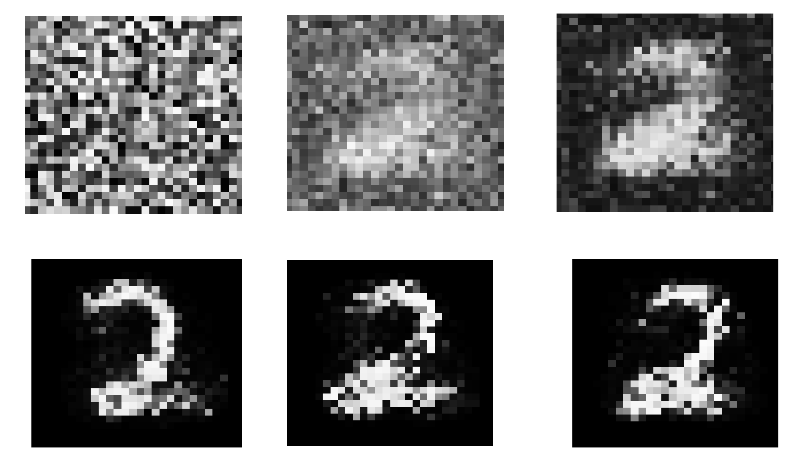
\includegraphics[width=1\textwidth]{images/08-DCGAN}\caption{Résultats d'un apprentissage de 2 par un DCGAN basique avec des couches à convolutions dans les premières couches des réseaux.)}
\end{center}
\end{figure} 

\section{Échanges avec Giuseppe Valenzise}
Dans le domaine d'évaluation de la qualité des images, on distingue l'estimation avec référence (comparaison par rapport à une image) de l'estimation sans référence.
Maître de conférences au laboratoire L2S de CentraleSupélec, Giuseppe Valenzise est spécialiste en évaluation de qualité d'image (\textit{Visual Quality Assessment}) sans référence.
Les conclusions auxquelles nous avons pu aboutir au cours de l'échange étaient les mêmes que celles que nous avions pu formuler par le passé. Cela a néanmoins permis de les clarifier, et de nous confirmer l'intérêt du Wasserstein GAN. 
\begin{itemize}
\item L'évaluation d'une qualité d'image standard passe très souvent par l'usage de métriques (i.e. fonctions) appliquées sur les valeurs des pixels. Une métrique souvent proposée est NIQE (\textit{Naturalness Image Quality Evaluator}), qui consiste en la recherche de statistiques gaussiennes locales avec des coefficients mscn (\textit{mean subtracted and contrast normalized}). Néanmoins, les images utilisées dans notre étude (MNIST, CIFAR) sont beaucoup plus petites que des images standard (28x28 et 32x32 au lieu de plusieurs millions de pixels par image). L'estimation des gaussiennes est fortement bruitée, les métriques ne sont donc pas efficaces.
\item Les méthodes avancées d'évaluation de qualité d'image consistent en l'utilisation de classificateurs. On cherche à extraire des caractéristiques des images (vecteurs, symétries, ...) et on crée des classificateurs qui décident sur la base de ces caractéristiques. Le travail consiste alors à trouver les meilleures caractéristiques d'image.
\item Dans le cas des réseaux neuronaux, la distance entre les poids du réseau constitue une des caractéristiques les plus exploitées. G. Valenzise considère que dans le cas du GAN, la fonction de coût du discriminateur devrait constituer un des meilleurs classificateurs. Or dans le cas d'un GAN classique, nous avons pu remarquer qu'elle ne suit pas toujours la qualité des images.
\item Il nous a suggéré de réfléchir à un « réseau de classification » qui permettrait de s'affranchir de ces problèmes. Or, un tel réseau de classification existe déjà dans la littérature : Le WGAN.  
\item Le WGAN permet d'obtenir un meilleur lien entre qualité d'image et fonction de coût du discriminateur, le classificateur \textit{fonction de coût du réseau discriminant} est amélioré, en modifiant profondément sa structure.
\end{itemize}

\section{Pistes de recherche}
Cette section regroupe les pistes de recherche que nous avons pu rencontrer mais qui n'ont pas été approfondie faute de temps. Certaines pistes de recherches ne bénéficient pas de papiers à leur sujet.
\begin{itemize}
\item Étudier l’impact du nombre d’images disponibles dans la base d’entraînement. A priori, s’il est petit, l’effet d’apprentissage « par cœur » peut apparaître. Proposé par la chef de l’équipe de TaO du LRI.
\item GAN à secousses. Le groupe Salamandre \cite{bouvier_dyvoire_dessine-moi_2018} s'y est intéressé de plus près.
\end{itemize}

\subsection{Generative Adversarial Networks 1D : Visualisation en une dimension}
\label{gan1D}
Afin de mieux comprendre le fonctionnement du GAN, nous nous sommes intéressés à l'étude du GAN à une dimension.  Le principe consiste à remplacer la banque d'image, de dimension 784, par des entrées à une dimension. On peut l'interpréter comme un scalaire, ou comme un pixel. La distribution représentée $p_{data}$ est alors une distribution unidimensionnelle, que nous allons pouvoir représenter graphiquement, plutôt qu'une distribution à 784 dimensions.

Les résultats ne furent pas concluants. En effet, la distribution du générateur ne s'approche pas du tout de la représentation $p_{data}$ comme on peut le voir à la figure \ref{fig:gan1D}. On fait figurer en noir la distribution cible $p_{data}$, en bleu le score attribué par le discriminateur, et en rouge un histogramme des résultats du Générateur.

\begin{figure}[h!]
\begin{center}
\minipage{0.32\textwidth}
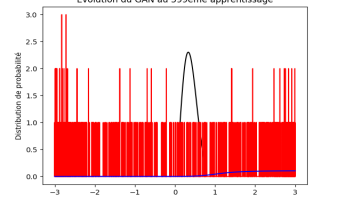
\includegraphics[width=1\textwidth]{images/Gan1D-1.png}
\centering\\Instant initial.
\endminipage\hfill
\minipage{0.32\textwidth}
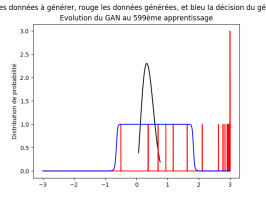
\includegraphics[width=1\textwidth]{images/Gan1D-4.png}
\centering\\Apprentissage en cours
\endminipage\hfill
\minipage{0.32\textwidth}
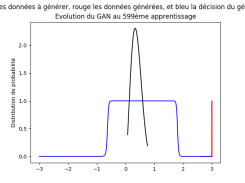
\includegraphics[width=1\textwidth]{images/Gan1D-5.png}
\centering\\après un certain nombre d'apprentissage.
\endminipage\hfill
\caption{Graphique du GAN 1D.  La distribution prend ses valeurs entre -3 et 3}
\label{fig:gan1D}
\end{center}
Initialement la distribution $p_{G}$ est une distribution uniforme, ce qui est conforme aux attentes considérant que les poids du réseau sont initialisés suivant une loi uniforme. Après apprentissage, le discriminateur cherche à faire apprendre une distribution proche de $p_{data}$. Néanmoins, après un nombre supérieur d'apprentissage, le générateur est perdu. Dans notre cas, l'interprétation est la suivante : le générateur est allé dans un minimum local qui ne correspond pas au minimum que l'on cherche à atteindre. 
\end{figure}


 


